% !TeX program = lualatex
% !TeX encoding = UTF-8

\documentclass[x11names, border=5pt]{standalone}

\usepackage{siunitx}
\usepackage{tikz}
\usepackage{pgfplots}
\usepackage{drawproton}

\usetikzlibrary{calc, fadings, shadings, shadows}
\usepgfplotslibrary{units}
\pgfplotsset{compat=newest, filter discard warning=false, tick scale
binop=\times}

\tikzset{
	xq2shading/.style={
		rounded corners=5pt,
		drop shadow,
		preaction={fill=white, draw=black, line width=0.2pt},
		opacity=0.15,
		top color=red!70!magenta,
		bottom color=cyan,
		middle color=red!70!magenta!50!cyan!30!white,
		shading angle=45
	}
}

\pgfplotstableread[col sep=comma,
header=true]{datafiles/pdfdataQ200.csv}\pdfdatatableA
\pgfplotstableread[col sep=comma,
header=true]{datafiles/pdfdataQ210.csv}\pdfdatatableB

\begin{document}

% Parton evolution visualisation only
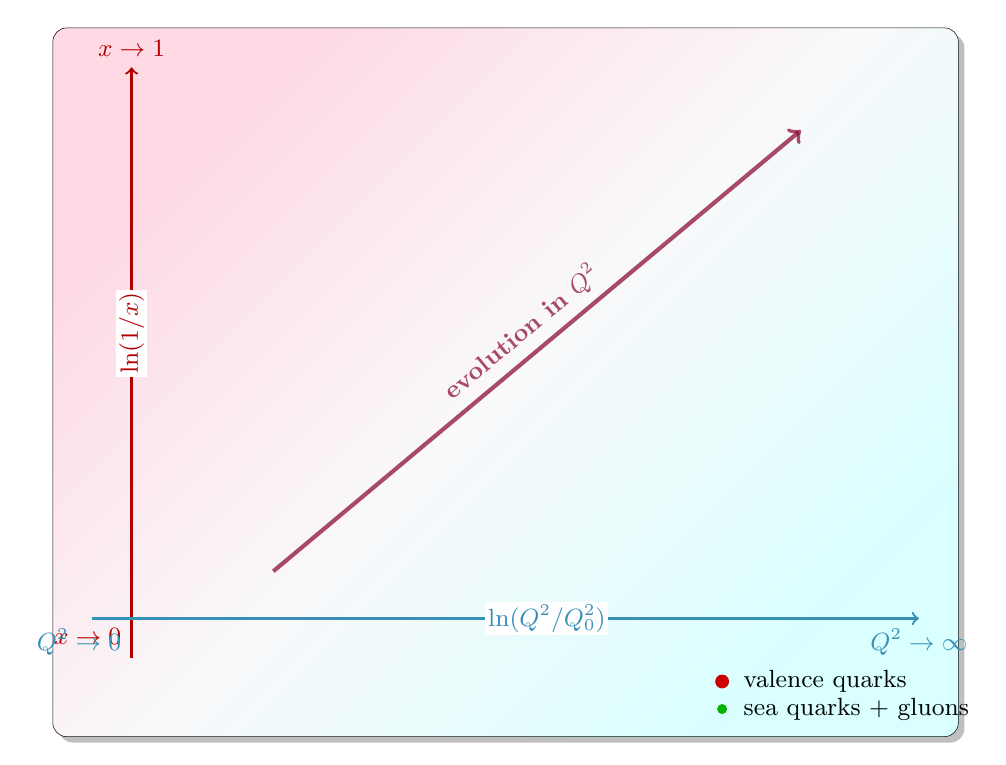
\begin{tikzpicture}
	\path[xq2shading] (-1.0,7.5) rectangle (10.5,-1.5);

	% Axes with labels
	\draw[->, red!70!black, line width=0.8pt]
	(0,-0.5) -- (0,7)
	node[at={(0,0)}, below left, font=\small] {\(x \to 0\)}
	node[at={(0,7)}, above, font=\small] {\(x \to 1\)}
	node[pos=0.55, rotate=90, font=\small, fill=white, inner sep=1pt]
	{\(\ln(1/x)\)};
	\draw[->, cyan!70!black, line width=0.8pt]
	(-0.5,0) -- (10,0)
	node[at={(0,0)}, below left, font=\small] {\(Q^2 \to 0\)}
	node[at={(10,0)}, below, font=\small] {\(Q^2 \to \infty\)}
	node[pos=0.55, font=\small, fill=white, inner sep=1pt]
	{\(\ln(Q^2/Q_0^2)\)};

	% Evolution arrow (diagonal)
	\draw[->, very thick, purple!70!black, opacity=0.7, line width=1.5pt]
	(1.8, 0.6) -- (8.5, 6.2)
	node[midway, above, sloped, font=\small]
	{\textbf{evolution in \(Q^2\)}};

	% Proton grid
	\begin{scope}[scale=0.8, xshift=50pt, yshift=30pt]
		\foreach \iprotonx in {0,...,3} {
			\foreach \iprotonq in {0,...,3} {
				\begin{scope}[xshift={90*\iprotonq*1pt}, yshift={60*\iprotonx*1pt}]
					\pgfmathsetmacro{\protonradius}{15*(1+0.3*sqrt(\iprotonx+4*\iprotonq/3))}
					\pgfmathsetmacro{\nValence}{max(1, \iprotonx + 1)}
					\pgfmathsetmacro{\nSea}{max(1, \iprotonq + 1)}
					\drawproton{\protonradius}{\nValence}{\nSea}
				\end{scope}
			}
		}
	\end{scope}

	% Legend for partons
	\begin{scope}[shift={(7.5, -0.8)}]
		\fill[red!80!black] (0, 0) circle (2.5pt);
		\node[right, font=\small] at (0.15, 0) {valence quarks};
		\fill[green!70!black] (0, -0.35) circle (1.8pt);
		\node[right, font=\small] at (0.15, -0.35) {sea quarks + gluons};
	\end{scope}
\end{tikzpicture}

\pagebreak

% Parton evolution + data visualisation
\begin{tikzpicture}
	\begin{scope}[yscale=0.4, xslant=0.6,
		every node/.append style={transform shape}]
		\path[xq2shading] (-1.0,7.5) rectangle (10.5,-1.0);
		\draw[->, red!70!black] (0,-0.5) -- (0,7)
		node[pos=0.5, rotate=90, font=\small] {\(\ln(1/x)\)};
		\draw[->, cyan!70!black] (-0.5,0) -- (10,0)
		node[pos=0.5, font=\small] {\(\ln(Q^2/Q_0^2)\)};
		\node[red!70!black, font=\small\bfseries]  at (5,7.2) {high-energy
		collisions};
		\node[cyan!70!black, rotate=-90, font=\small\bfseries] at
		(10.2,3.5) {high momentum transfer};

		\begin{scope}[scale=0.8, xshift=50pt, yshift=30pt]
			\foreach \iprotonx in {0,...,3} {
				\foreach \iprotonq in {0,...,3} {
					\begin{scope}[xshift={90*\iprotonq*1pt}, yshift={60*\iprotonx*1pt}]
						\pgfmathsetmacro{\protonradius}{15*(1+0.3*sqrt(\iprotonx+4*\iprotonq/3))}
						\pgfmathsetmacro{\nValence}{max(1, \iprotonx + 1)}
						\pgfmathsetmacro{\nSea}{max(1, \iprotonq + 1)}
						\drawproton{\protonradius}{\nValence}{\nSea}
						\coordinate (proton\iprotonx\iprotonq) at (0,0);
					\end{scope}
				}
			}
		\end{scope}
	\end{scope}

	% PDF plots overlaid
	\begin{scope}[yslant=0.66666666, scale=0.8, overlay]
		\begin{axis}[
				legend to name={leg:pdflegend},
				legend columns=1,
				legend style={cells={anchor=mid west}},
				at={(proton01)},
				scale only axis=true, width=108pt, height=108pt,
				xmode=log, xmax=1, xmin=1e-4, ymin=1e-3, ymax=5,
				clip=false,
				axis background/.style={fill=white, fill opacity=0.7},
				x tick label style={opacity=0.5},
				x dir=reverse
			]
			\addplot[black, thick]      table[x index=0,y index=2] {\pdfdatatableA};
			\addplot[blue]              table[x index=0,y index=3] {\pdfdatatableA};
			\addplot[red]               table[x index=0,y index=4] {\pdfdatatableA};
			\addplot[orange]            table[x index=0,y index=5] {\pdfdatatableA};
			\addplot[green!50!black]    table[x index=0,y index=6] {\pdfdatatableA};
			\node[below left, font=\small] at (rel axis cs:0.95,0.95)
			{\(Q^2 = \SI{10}{GeV^2}\)};
			\addlegendentry{gluon}
			\addlegendentry{up}
			\addlegendentry{down}
			\addlegendentry{antiup}
			\addlegendentry{antidown}
		\end{axis}

		\begin{axis}[
				at={(proton02)},
				scale only axis=true, width=108pt, height=108pt,
				xmode=log, xmax=1, xmin=1e-4, ymin=1e-3, ymax=5,
				clip=false,
				axis background/.style={fill=white, fill opacity=0.7},
				x tick label style={opacity=0.5},
				x dir=reverse
			]
			\addplot[black, thick]      table[x index=0,y index=2] {\pdfdatatableB};
			\addplot[blue]              table[x index=0,y index=3] {\pdfdatatableB};
			\addplot[red]               table[x index=0,y index=4] {\pdfdatatableB};
			\addplot[orange]            table[x index=0,y index=5] {\pdfdatatableB};
			\addplot[green!50!black]    table[x index=0,y index=6] {\pdfdatatableB};
			\node[below left, font=\small] at (rel axis cs:0.95,0.95)
			{\(Q^2 = \SI{100}{GeV^2}\)};
		\end{axis}
	\end{scope}

	% Axis title
	\path[scale=0.8] (proton01) +(0,108pt)
	node[above left, transform shape, font=\small] {\(x f(x, Q^2)\)};

	% Show legend
	\node[anchor=north west, font=\small] at (11, -1)
	{\pgfplotslegendfromname{leg:pdflegend}};
\end{tikzpicture}
\end{document}
